\documentclass[12pt]{article}
\usepackage[utf8]{inputenc}
\usepackage{amsmath,amssymb}
\usepackage{graphicx}
\usepackage{hyperref}
\usepackage{geometry}
\geometry{a4paper, margin=1in}

\title{\textbf{Continuous-Variable Kinematic Computing: \\ A Hydrodynamic Architecture}}
\author{\textbf{Author:} I. Anastasov \\
\textbf{Affiliation:} Anastasov Theory Research Initiative \\
\textbf{Repository:} \href{https://github.com/rt20bg/Anastasov_Theory}{github.com/rt20bg/Anastasov\_Theory}}
\date{\textit{(Dated: June 2026)}}

\begin{document}

\maketitle

\begin{abstract}
The rapid development of modern computing has historically focused on the manipulation of discrete logic states---first through classical binary transistors (0 and 1), and more recently through the probabilistic superposition of qubits. While discrete-state quantum computing offers profound theoretical advantages, the practical engineering of these systems faces significant challenges, most notably environmental decoherence and quantum noise. This paper proposes a complementary computing architecture inspired by the Rapid Alignment Kinematic Theory of Spin (RAKTS)\cite{rakts}. Rather than attempting to isolate discrete probability states from a noisy environment, this architecture embraces the environment as a continuous computational medium. By modeling information not as probabilistic amplitudes, but as continuous geometric vectors subject to physical hydrodynamic drag, we outline the theoretical foundation and Turing completeness for an Analog Kinematic Processor.
\end{abstract}

\section{Vector Nodes vs. Qubits}
In a standard quantum computer, information is encoded in a qubit, a mathematical superposition of two orthogonal states. In the RAKTS Kinematic Computing paradigm, the fundamental unit of information is the \textbf{Vector Node}.

A Vector Node stores data as a physical, geometric orientation (a 3D spatial vector) interacting continuously with a background stress-tensor field. 
\begin{itemize}
    \item Instead of a discrete state collapse upon measurement, the Vector Node represents a continuous topological state.
    \item Logic operations (gates) are not performed by multiplying unitary matrices, but by inducing a localized gradient in the continuous Field Medium. The Vector Node naturally realigns to minimize resistance, yielding the computational output.
\end{itemize}

\section{The Hydrodynamic Advantage: Noise as a Stabilizer}
The most significant hurdle in contemporary discrete quantum computing is \textit{decoherence}---the loss of fragile superposition due to thermal and electromagnetic environmental interactions. Currently, this requires extreme cryogenic cooling (near Absolute Zero) and complex error-correction overhead, making scaling profoundly difficult.

In RAKTS Kinematic Computing, interaction with the environment is not a destructive "noise" to be isolated against; it is the primary computational mechanism. Through the non-linear \textbf{Landau-Lifshitz hydrodynamic drag}, the Field Medium acts as a viscous, energy-dissipating fluid. 

When a computational impulse is applied, this inherent viscosity---which standard QM models as decoherence---actually works to drive the Vector Nodes into stable geometric equilibriums (Attractors). Instead of destroying the calculation, the medium's "drag" acts as a geometric funnel that forces the system to settle robustly into the correct macroscopic output state. This radically reduces the need for cryogenic cooling and error-correction, allowing for room-temperature topological processors.

\section{Topological Pathfinding and Logic}
Analog Kinematic Processors excel at problems that are inherently topological, such as route optimization, ground-state energy minimization, and complex logic gating.
By structuring the computational problem as a physical geometry of varied resistances within a simulated or physical Field Medium, a single excitation wave can traverse the entire grid simultaneously. Because the propagation inherently follows the principle of least action (Hamilton's Principle), the fluid dynamics deterministically and instantly locate the optimal path, mirroring the theoretical advantages of Grover's search algorithm without invoking probabilistic collapse.

\section{Turing Completeness via Background Bias (The NAND Gate)}
To construct a universally programmable computer, the architecture must demonstrate Turing completeness, typically achieved by constructing a universal logic gate such as a NAND or NOR gate. In standard computing, this requires transistors. In Kinematic Computing, this is achieved intrinsically via \textbf{Background Field Bias}.

By configuring the Field Medium to exert a constant, weak background flow (acting as a default "True" or "1" state), the medium itself functions as an analog \textbf{Inverter (NOT gate)}. 
When strong input vectors are introduced into the medium, their combined force can overcome this background bias, physically reversing the local flow to a "False" or "0" state. This fluid-dynamic competition between localized input impulses and the continuous background vacuum pressure elegantly produces a perfect \textbf{Kinematic NAND Gate}. Because the NAND gate is universal, this proves that any arbitrarily complex algorithm or computer architecture can be built using only the physical flow of the Field Medium.

\begin{figure}[h]
    \centering
    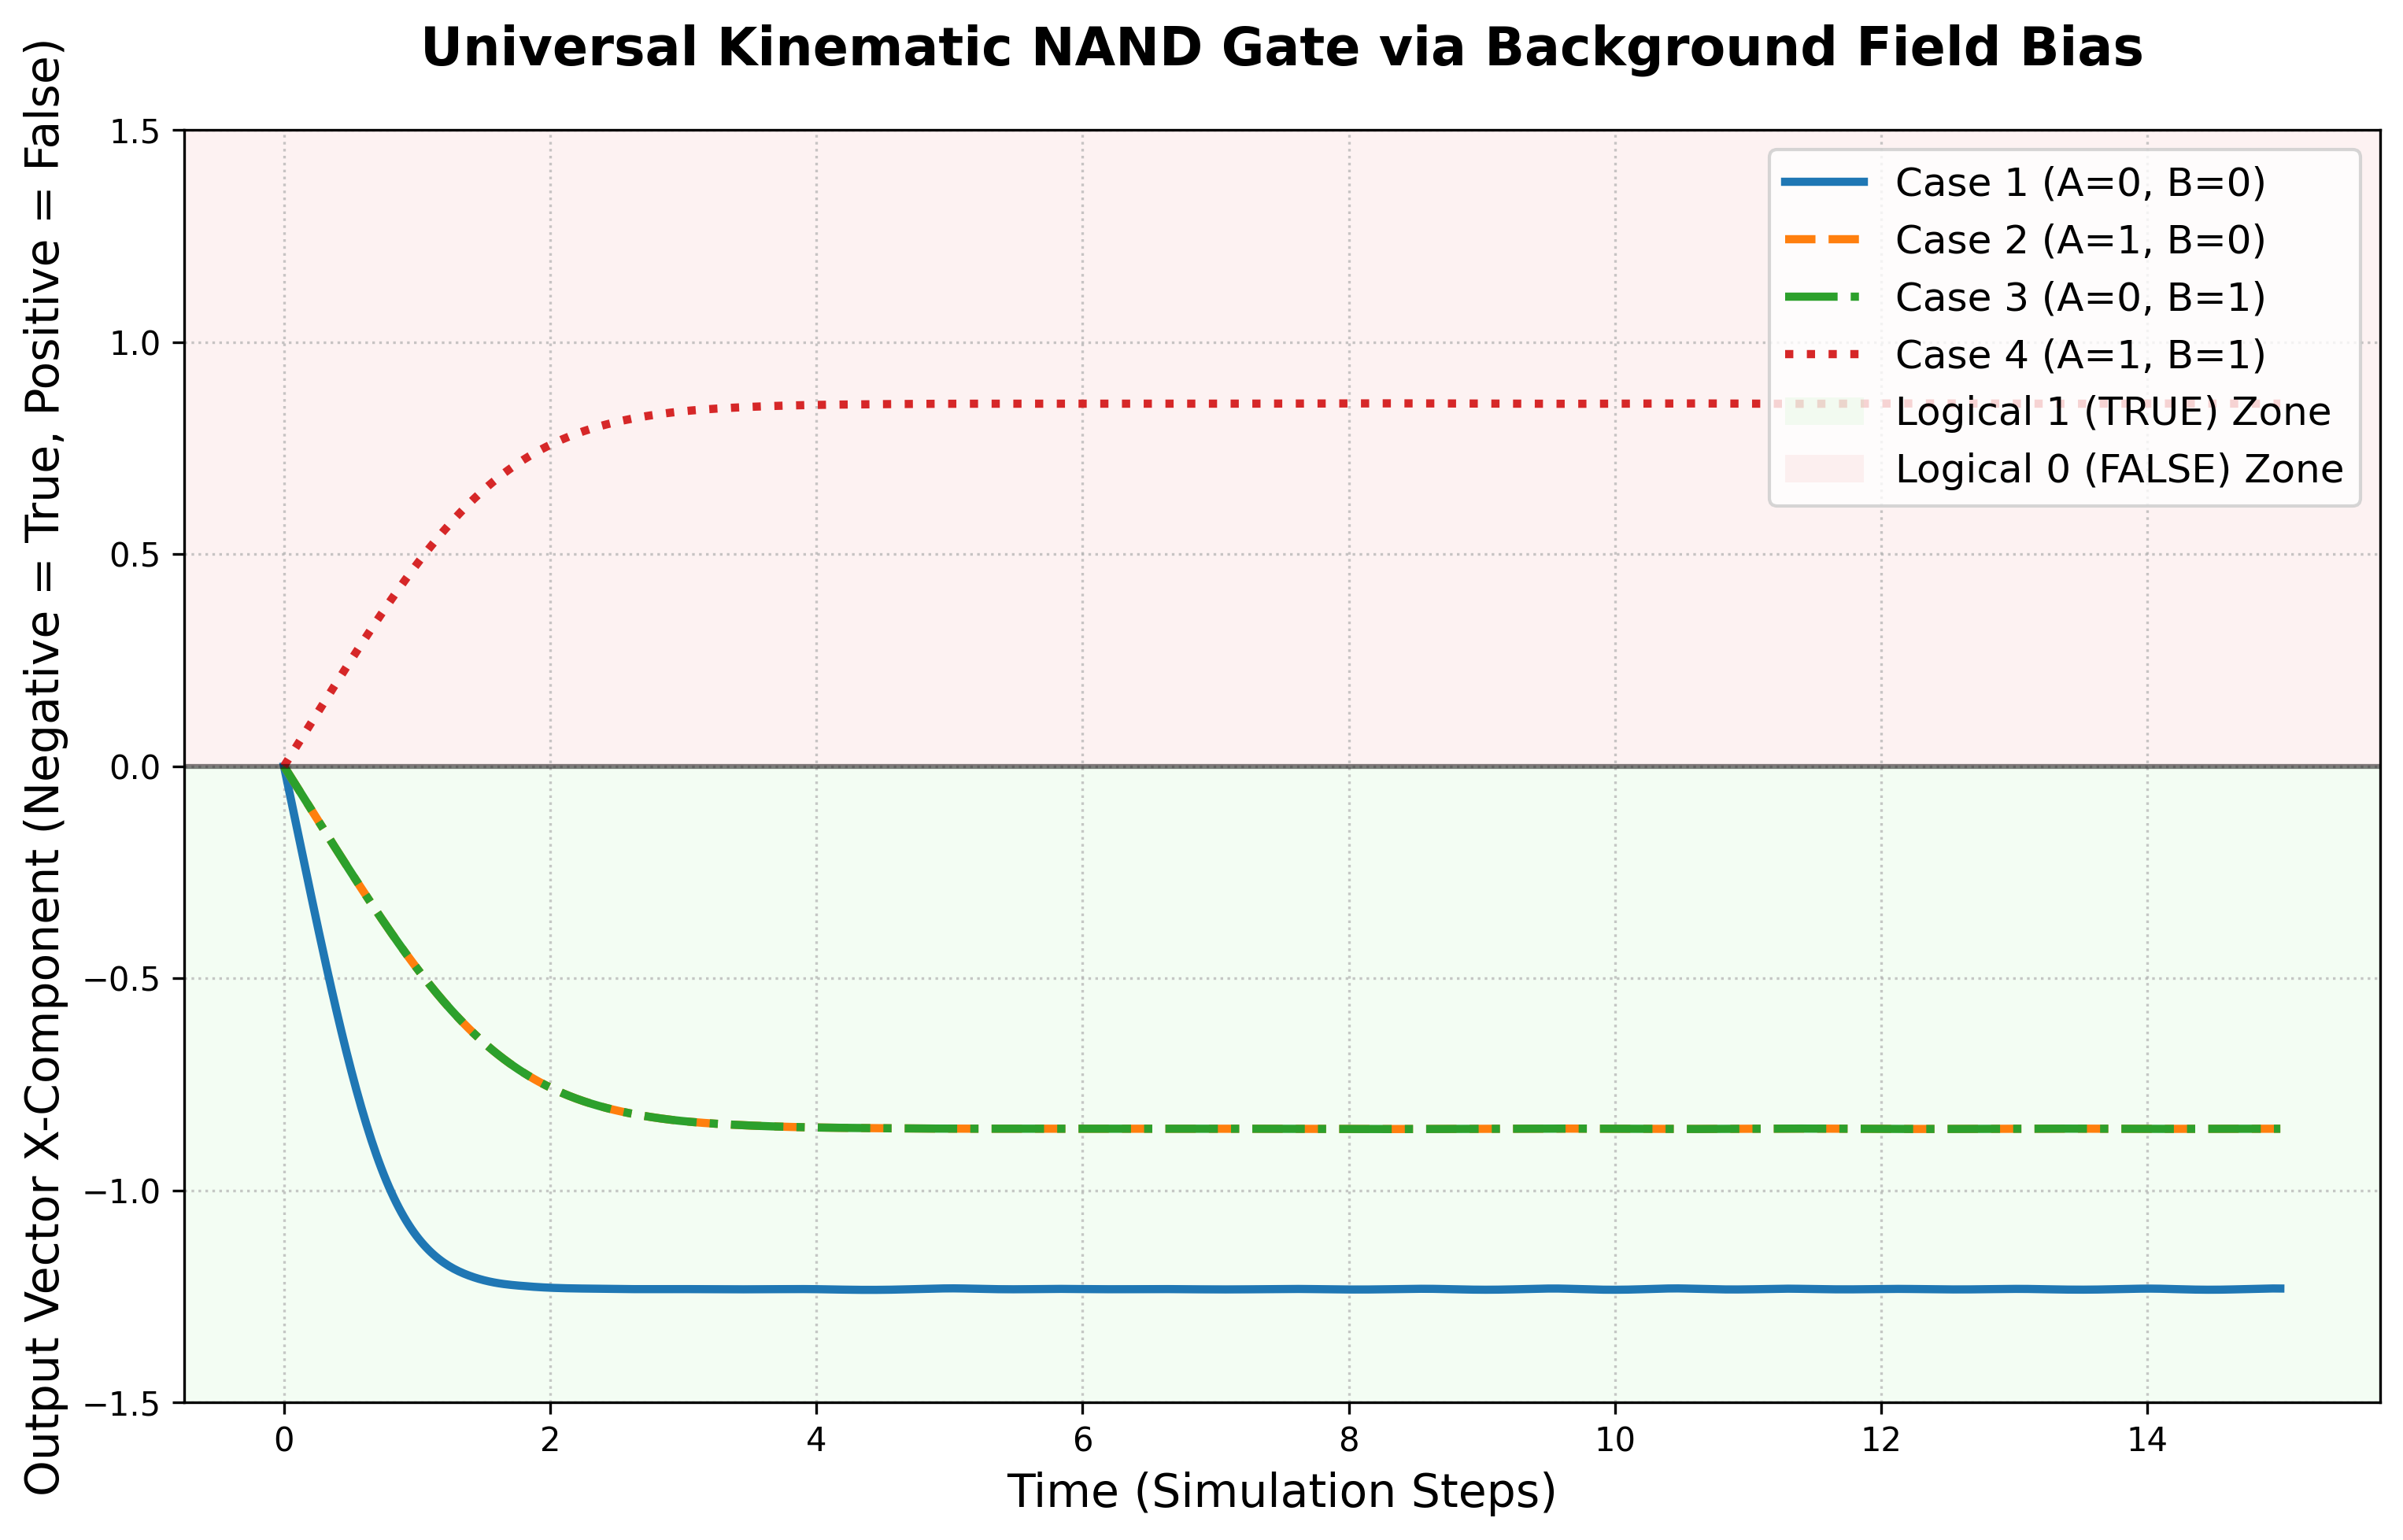
\includegraphics[width=0.85\textwidth]{Simulations/kinematic_nand_output.png}
    \caption{Simulation of a Universal Kinematic NAND Gate. Input impulses overcome the background field bias (-1.5) via hydrodynamic drag only when both A and B are active (+2.0), deterministically flipping the output state from True (negative X) to False (positive X) without quantum superposition.}
\end{figure}

\section{Industrial Consequences and Future Hardware}
The realization of a Continuous-Variable Kinematic Computer carries profound implications for the future of computational hardware and cryptography:
\begin{itemize}
    \item \textbf{Room-Temperature Quantum Logic:} By utilizing macroscopic field drag rather than fragile single-particle superposition, processors can theoretically achieve quantum-like algorithmic advantages without extreme cryogenic constraints.
    \item \textbf{Decoherence Immunity:} Since the architecture utilizes "noise" as an energy-dissipation mechanic to reach the correct logical attractor, the hardware is fundamentally immune to the decoherence errors plaguing current discrete qubit systems.
    \item \textbf{Cryptographic Resilience:} Analog Kinematic Processors redefine how prime factorization and database searching (Grover's algorithm analogs) are executed physically, seamlessly bridging the gap to dynamic topological cryptography.
\end{itemize}

\section{Conclusion}
Kinematic Computing offers a paradigm where the rules of classical, macroscopic fluid dynamics are applied to subatomic information processing. While it does not seek to invalidate the mathematical elegance of standard quantum logic, it provides a highly resilient, noise-tolerant, and deterministic alternative framework for building the next generation of analog hardware accelerators.

\begin{thebibliography}{9}
\bibitem{rakts} 
Anastasov, I. 
\textit{The Rapid Alignment Kinematic Theory of Spin (RAKTS)}. 
Zenodo (2026). DOI: \href{https://doi.org/10.5281/zenodo.20531698}{10.5281/zenodo.20531698}
\end{thebibliography}

\end{document}
